\section[Introdução]{Introdução}

O projeto \textbf{ENSportive} é um sistema web desenvolvido para a \textbf{Escola de Raquetes ENSportive},
com o objetivo de gerenciar os processos internos da escola, como cadastro de alunos, professores
e planos, controle de horários de aula, reposições e feedbacks. O sistema foi construído como
parte de um ecossistema maior da ENSportive, focando exclusivamente na Escola de Raquetes para
garantir a entregabilidade dentro do semestre.

\textbf{Stakeholders:} Representantes da ENSportive, responsáveis pela definição dos requisitos
e validação dos protótipos ao longo do projeto.

\textbf{Período de Execução:} 2024/1.

\begin{figure}[H]
    \centering
    \small
    \caption{Time ENSportive}
    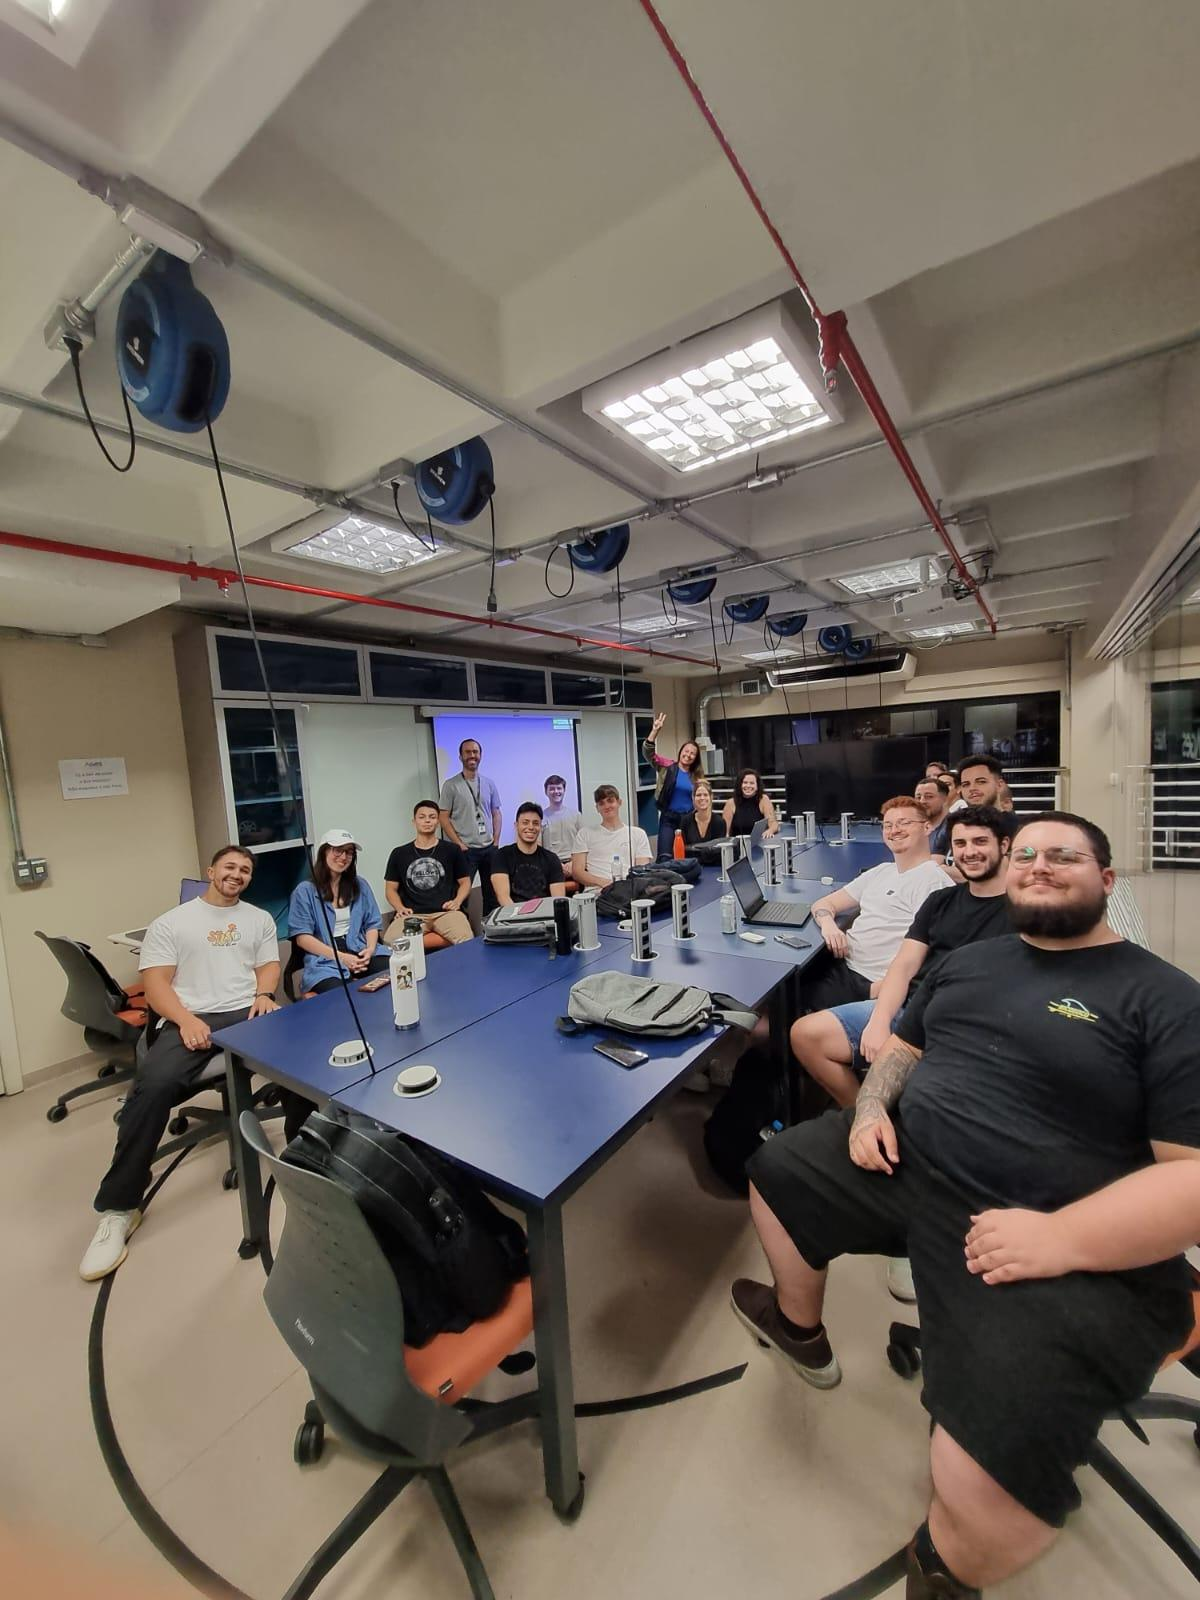
\includegraphics[width=1\linewidth]{conteudo//2 - ages I//conteudo//figures/TimeENSportive.jpeg}
    Fonte: Arquivos pessoais
    \label{fig:ensportive-time}
\end{figure}